\PassOptionsToPackage{unicode}{hyperref}
\PassOptionsToPackage{naturalnames}{hyperref}
\documentclass{beamer} 
%\usepackage{babel}
%\usepackage[utf8]{inputenc}


%%% FONT SELECTION %%%%%%%%%%%%%%%%%
%%% we choose a sans font %%%%%%%%%%
%\usepackage{kmath,kerkis} 
%\usepackage[default]{gfsneohellenic} 
%%%%%%%%%%%%%%%%%%%%%%%%%%%%%%%%%%%%

\usepackage{color}
\usepackage{amsmath}
\usepackage{amssymb}

\usepackage{epstopdf}
\usepackage{graphicx}

\usepackage{mathtools}
\usepackage{graphicx}

\usepackage[utf8]{inputenc}
\usepackage{float}

\usepackage{amsthm}
\usepackage{mathtools}
\usepackage{amsfonts}

\usepackage{amssymb}
\usepackage{gensymb}

\usepackage{braket}


\renewcommand{\r}{\mathbf{r}}

\graphicspath{{./images/}}

%%
% load TEI-Pel - specific layout
\usepackage{TeiPel_En_Beamer_Layout}
\setTeipelLayout{draft,newlogo}% options: "draft", "newlogo"

%%%%%%%%%%%%%%%%%%%%%%%%%%%%%%%%%%%%%%%%%%%%%%%%%%%%%%%%%%%%
% Thesis Info %%%%%%%%%%%%%%%%%%%%%%%%%%%%%%%%%%%%%%%%%%%%%%
%%%%%%%%%%%%%%%%%%%%%%%%%%%%%%%%%%%%%%%%%%%%%%%%%%%%%%%%%%%%
    % title
        \title[This is my Title]{Generation and manipulation\\ of entangled photon pairs \\ in coupled resonators}  
    % author 
    % (In the mandatory argument "{}", separate multiple
    % authors with "\and" - use "\\" for better author name formatting
    % in the title page. In the optional argument "[]" include all
    % author names, with no "\and" or text formatting macros.)
    % Example: 
    %\author[A. Author Albert Einstein]{Anthony Author \and Albert Einstein}
        \author[Marco Canteri]{Marco Canteri}
    % supervisor    
        \supervisor{Supervisors}{Prof. Lorenzo Pavesi}{Dott. Massimo Borghi}
    % date
        \presentationDate{July 19, 2017}
%%%%%%%%%%%%%%%%


\setbeamertemplate{caption}{\raggedright\insertcaption\par}
\begin{document}

% typeset front slides
    \typesetFrontSlides

%%%%%%%%%%%%%%%%
% Your Slides Start here:

%%%%
\section{Introduction}
\subsection{Aim of the thesis}
\begin{frame}[plain]{Aim of the thesis}
\begin{figure}
\centering
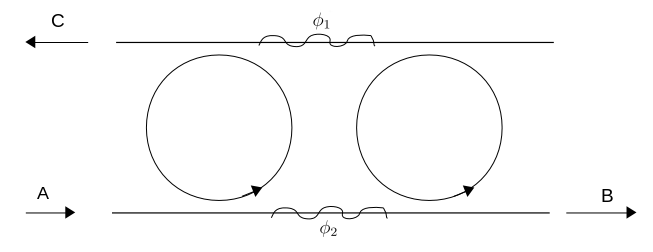
\includegraphics[width =.8\textwidth]{structure}
\end{figure}
\begin{itemize}
\item Input coherent state
\item Field Enhancement
\item Spontaneous Four Wave Mixing $\implies$ photons generation
\item Heaters can change the phases $\implies$ manipulation
\item Output states

\end{itemize}
\end{frame}

\subsection{Basic blocks}
\begin{frame}[plain]{Silicon photonic}
\begin{figure}[H]
\centering
\begin{minipage}{.5\textwidth}
\centering
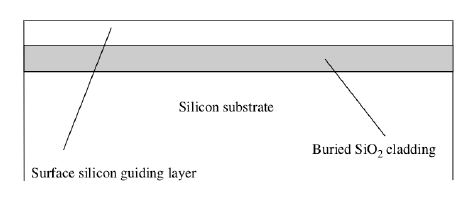
\includegraphics[width =\textwidth]{SOIstructure}
\end{minipage}%
\begin{minipage}{.5\textwidth}
\centering
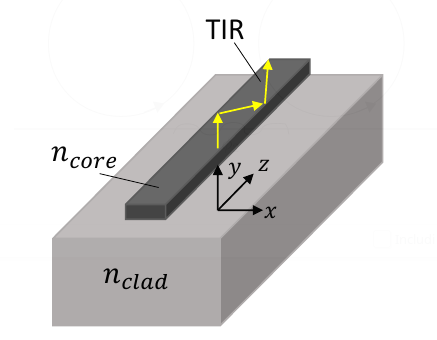
\includegraphics[width =.7\textwidth]{slab}
\end{minipage}
\end{figure}
\centering
Typical dimension: %ubstrate $\simeq 700 \mu m$\\ cladding $\simeq \mu m$\\ core $\simeq 10^2 $ nm
\begin{tabular}{cc}
            substrate & $\simeq 700 \mu m$\\

             cladding & $\simeq \mu m$\\

            core & $\simeq 10^2 $ nm
        \end{tabular}

\end{frame}


\begin{frame}[plain]{Resonator APF}
\begin{figure}
\centering
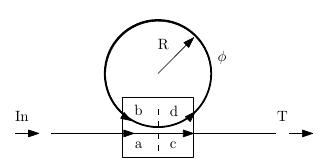
\includegraphics[width =.7\textwidth]{APF}
\end{figure}
\vspace{2em}
Constructive interference $n_{eff} L = m \lambda_m \implies$ field enhancement $\implies$ non linear effects
\end{frame}

\begin{frame}[plain]{Coupling}
Gap in the order of $\simeq$ 100 nm $\implies$ evanescent field \\
In quantum mechanics $\implies$ quantum tunneling\newline
\\Mathematically can be treated as a Quad port beam splitter
\begin{equation}\begin{pmatrix}c \\ d \end{pmatrix} = \begin{pmatrix}r &ik\\ ik &r \end{pmatrix}
 \begin{pmatrix}a\\b \end{pmatrix}\end{equation}
$r$ reflection coefficient, $k$ transmission coefficient $k^2+r^2=1$
\end{frame}

\begin{frame}[plain]{Resonator APF}
with the roundtrip phase condition \[b = e^{-\alpha 2\pi R} e^{-i\beta 2\pi R}d \equiv\tau e^{-i\phi(\lambda)}d\] the Transfer function can be found
\begin{equation}H_{AP} = \frac{c}{a} = \frac{\tau - re^{i\phi(\lambda)}}{r\tau -e^{i\phi(\lambda)}}\end{equation}
\end{frame}

\begin{frame}[plain]{Resonator ADF}
\begin{figure}
\centering
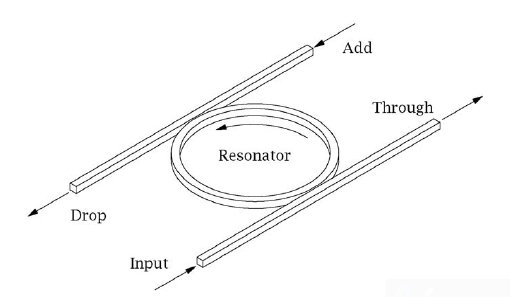
\includegraphics[width =.6\textwidth]{ADFfigo}
\end{figure}
\vspace{2em}
\begin{equation}H^T_{AD} = \frac{k^2\sqrt{\tau} e^{i\phi/2}}{r^2\tau -e^{i\phi}}\qquad H^D_{AD}  = \frac{r(e^{i\phi} - \tau)}{e^{i\phi}-r^2\tau} \end{equation}
\end{frame}



\begin{frame}[plain]{Transfer function}
\begin{figure}
\centering
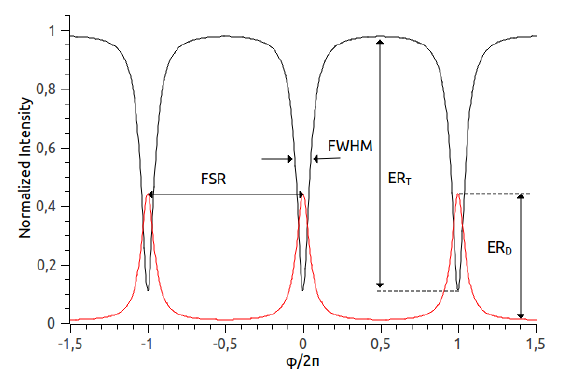
\includegraphics[width =.8\textwidth]{transferfunction}
\end{figure}
\end{frame}


\begin{frame}[plain]{Coupled resonators}
\begin{figure}
\centering
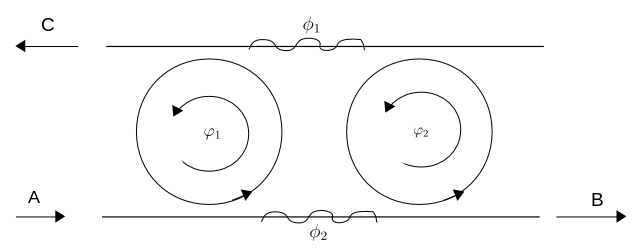
\includegraphics[width =.6\textwidth]{coupled}
\end{figure}
\vspace{2em}
The most important quantities are the field enhancements for the two rings, they need to be equal for both ring 
\[\phi_1 + \phi_2 = 2m\pi\]
\end{frame}


\begin{frame}[plain]{Field enhancements}
\begin{figure}[H]
\centering
\begin{minipage}{.5\textwidth}
\centering
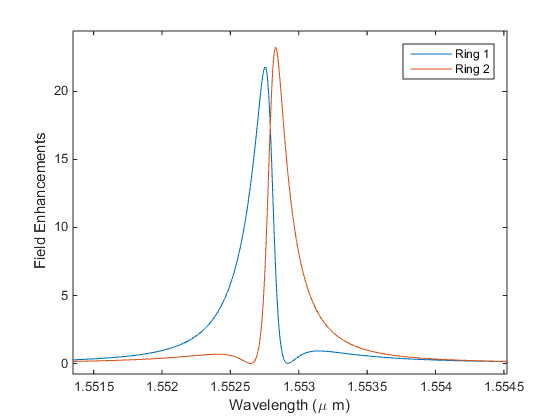
\includegraphics[width =\textwidth]{FE_fase_2pi}
\caption{$\phi_1+\phi_2 = 2\pi$}
\end{minipage}%
\begin{minipage}{.5\textwidth}
\centering
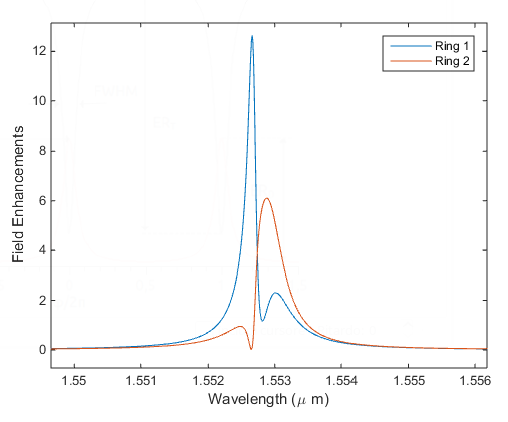
\includegraphics[width =.9\textwidth]{FE_fase_pi}
\caption{$\phi_1+\phi_2 = -\pi$}
\end{minipage}
\end{figure}
\end{frame}


\begin{frame}[plain]{Full expressions}
\[FE_1 = \frac{ie^{i(\varphi_1+\phi_2+\phi_1)}k (e^{i\varphi_2}-r^2\tau_2)-ie^{\frac{i}{2}(\varphi_1+\varphi_2)}k^3(k^2+r^2)\sqrt{\tau_1\tau_2}\tau L^2}{e^{i(\phi_1+\phi_2)}(e^{i\varphi_1}-r^2\tau_1)(e^{i\varphi_2}-r^2\tau_2)-e^{\frac{i}{2}(\varphi_1+\varphi_2)}k^4\sqrt{\tau_1\tau_2}\tau L^2}\]
\[FE_2 = \frac{ie^{i(\varphi_2+\phi_1)}kr (-e^{i\varphi_1}+(r^2+k^2)\tau_1)\tau L}{e^{i(\phi_1+\phi_2)}(e^{i\varphi_1}-r^2\tau_1)(-e^{i\varphi_2}+r^2\tau_2)+e^{\frac{i}{2}(\varphi_1+\varphi_2)}k^4\sqrt{\tau_1\tau_2}\tau L^2}\]
\end{frame}




\section{Physical framework}
\subsection{Non linear optics}
\begin{frame}[plain]
NON LINEAR OPTICS
\end{frame}


\begin{frame}[plain]{Polarization}
In first approximation
\begin{equation}\label{linearP} \mathbf{P} = \varepsilon_0 \chi \mathbf{E}
\end{equation}
which can be expandend in 
\begin{equation}P_i  = \varepsilon_0(\sum_j \chi_{ij}^{(1)} E_j + \sum_{j,k}x_{ijk}^{(2)}E_jE_k + \sum_{j,k,l}\chi_{ijkl}^{(3)}E_jE_kE_l + \dots )\end{equation}
silicon is a centrosymmetric crystal $\implies$ $\chi^{(2)} = 0$, the first non-linear order is the third one: Kerr nonlinearity
\end{frame}


\begin{frame}[plain]{Polarization}
Wave equation can be written as 
\begin{equation}\label{wavesource}\left(\nabla^2 - \frac{n^2}{c^2}\frac{\partial^2}{\partial t^2}\right)E = \mu_0\frac{\partial^2 P_{NL}}{\partial t^2}\end{equation}
If we take \[E = \sum_{j=1}^{4} \frac{1}{2}(A_j(z)e^{i(\omega_jt -k_jz)}+\text{c.c})\] in $P_{NL} = \varepsilon_0\chi^{(3)}E^3$ there are terms
\[\sum_{l,j,m=\pm1,\pm2,\pm3,\pm4}\left(\frac{1}{8}A_lA_jA_l e^{i(\omega_l+\omega_j+\omega_m)t}e^{-i(k_l+k_j+k_m)z}\right)\]

       Non-linear polarization act as a source $\implies$ new frequencies arise

\end{frame}


\begin{frame}[plain]{Four Wave Mixing}
\begin{figure}
\centering
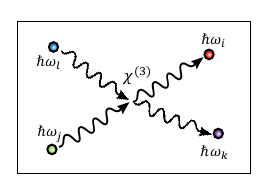
\includegraphics[width = .5\textwidth]{FWMphotons}
\end{figure}
Frequency of Four Wave Mixing $\omega_l = \omega_i - \omega_j +\omega_k$ phase matching condition $k_l = k_i - k_j +k_k$ \\
Can be seen as a simultaneous creation of two photons and an annhilation of two photons

\end{frame}

\begin{frame}[plain]{non degenerate Four Wave Mixing}
\begin{figure}
\centering
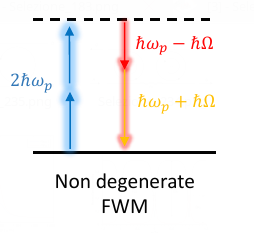
\includegraphics[width = .4\textwidth]{NondegFWM}
\end{figure}
$\omega_j = \omega_l \equiv \omega_p$ pump; $\omega_i\equiv \omega_s$;  signal $\omega_k \equiv \omega_i$ idler\\
In the classical description the process is stimulated, in the quantum figure is spontaneous
\end{frame}


\begin{frame}[plain]{Displacement field}
in a medium $\mathbf{D}$ is divergenceless $\implies$ it is more convenient to take $\mathbf{D}$ as our fundamental field
\begin{equation}P^i = \Gamma^{ij}_1D^j +\Gamma_2^{ijk}D^jD^k + \Gamma_3^{ijkl}D^jD^kD^l + \dots\end{equation}
summation implied
\begin{equation}\Gamma_3^{ijkl} = \frac{\chi_{ijk}^{(3)}}{\varepsilon_0 n^2(\omega_l)n^2(\omega_j)n^2(\omega_i)n^2(\omega_k)}\end{equation}
\end{frame}

\subsection{Quantum optics}
\begin{frame}[plain]{Field quantization}
The displacement field is quantizied and written in terms of the annhilation operator $a_k$ and the creation operator $a_k^\dagger$
\begin{equation}
\mathbf{D}(\r) = \sqrt{\frac{\hbar \omega_k}{2}}a_k \mathbf{D}_k(\r) + \sqrt{\frac{\hbar \omega_k}{2}}a_k^\dagger \mathbf{D}^*_k(\r)
\end{equation}
Linear Hamiltonian 
\begin{equation}H_L = \int dk \hbar \omega_k a_k^\dagger a_k  \end{equation}
\end{frame}

\begin{frame}[plain]{Coherent state}
Laser input state is a coherent state
\begin{equation}
\ket{\alpha} = e^{-\frac{1}{2}|\alpha|^2}\sum_{n=0}^{+\infty} \frac{\alpha^n}{\sqrt{n!}}\ket{n}
\end{equation}
$|\alpha|^2$ is the average photon number of the field.\\


\begin{equation}
\ket{\alpha} = \hat{D}(\alpha)\ket{vac}  = e^{\alpha a_k^\dagger -\text{H.c}} \ket{vac}
\end{equation}

generalized
\begin{equation}\hat{D}(\alpha) = e^{\alpha A^\dagger_P -\text{H.c}}\end{equation}
$A^\dagger_P = \int dk \phi_P(k) a_k^\dagger$, where $|\phi(k)|^2$ is the probability of finding a photon with wavevector $k$
\[\int dk |\phi_P(k)|^2 = 1\]
\end{frame}


\begin{frame}[plain]{Asymptotic field}
\begin{figure}
\centering
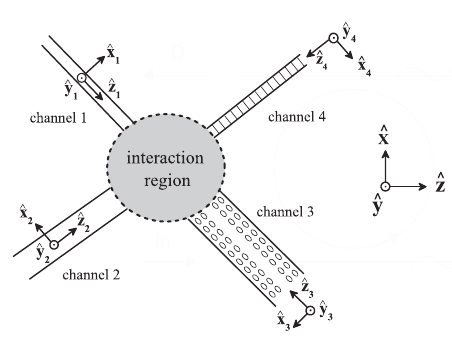
\includegraphics[width = .5\textwidth]{asymptotic}
\end{figure}
The idea behind this theory is to provide an easier way to study complex stuctures.\\
An asymptotic-in and an asymptotic-out state are introduced 

\end{frame}


\begin{frame}[plain]{Asymptotic-in}
\begin{figure}
\centering
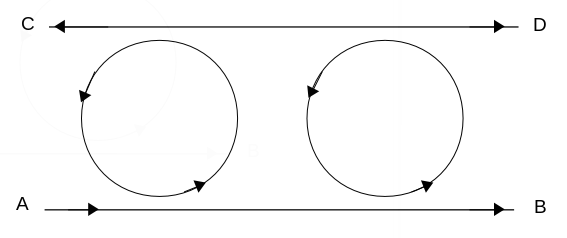
\includegraphics[width = .5\textwidth]{Asyina2}
\end{figure}
An asymptotic-in far from the interaction region corresponds to a wave incoming in channel $n$ and outgoing waves in every other channel

\begin{equation}\label{asyin}\mathbf{D}^{asy-in}_{n,k} \sim \mathbf{D}_{n,k}(\r_n) + \sum_{n'}\int_{0}^{+\infty}dk' T^{out}_{n,n'}(k,k')\mathbf{D}_{n',-k'}(r_{n'})\end{equation}

\end{frame}


\begin{frame}[plain]{Asymptotic-out}
\begin{figure}
\centering
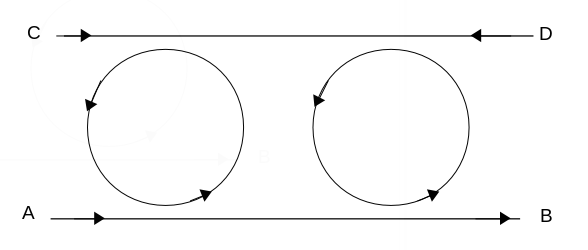
\includegraphics[width = .5\textwidth]{Asyoutb2}
\end{figure}
An asymptotic-out far from the interaction region corresponds to a wave outgoing in channel $n$ and incoming waves in every other channel
\begin{equation}\label{asyout}\mathbf{D}^{asy-out}_{n,k} \sim \mathbf{D}_{n,-k}(\r_n) + \sum_{n'}\int_{0}^{+\infty}dk' T^{in}_{n,n'}(k,k')\mathbf{D}_{n',k'}(r_{n'})
\end{equation} 

\end{frame}



\begin{frame}[plain]{Field operator}
we can write the field operator as a superposition of asymptotic-out fields
\begin{equation}\mathbf{D}(\r) = \sum_n \int_{0}^{+\infty}dk \sqrt{\frac{\hbar \omega_{n,k}}{2}}a_{n,k}\mathbf{D}_{n,k}^{asy-in}(\r) + \text{H.c}\end{equation}
\begin{equation}[a_{n,k},a_{n',k'}] = 0 \qquad [a_{n,k},a_{n',k'}^\dagger] = \delta_{nn'}\delta(k-k')\end{equation}
or asymptotic-out fields
\begin{equation}\label{dasyout}\mathbf{D}(\r) = \sum_n \int_{0}^{+\infty}dk \sqrt{\frac{\hbar \omega_{n,k}}{2}}b_{n,k}\mathbf{D}_{n,k}^{asy-out}(\r) + \text{H.c}\end{equation}
\begin{equation}[b_{n,k},b_{n',k'}] = 0 \qquad [b_{n,k},b_{n',k'}^\dagger] = \delta_{nn'}\delta(k-k')\end{equation}
With this approach the linear Hamiltonian can be written with the state of the whole structure, hence the linear Hamiltonian is diagonal
\end{frame}


\begin{frame}[plain]{Non linear Hamiltonian}
The non linear Hamiltonian is 
\begin{equation}H_{NL} = -\frac{1}{3\varepsilon_0}\int\Gamma^{ijkl}_3(\r)D^iD^jD^kD^l\,d\r\end{equation}
Since the asymptotic states are a complete basis we can expand $D$ either on the asympotic-out states, or on the asymptotic-in, we can choose to expand two fields of this equation in terms of the asymptotic-in and the other two in terms of the asympotic-out.
\end{frame}


\begin{frame}[plain]{Non linear Hamiltonian}
\begin{multline}H_{NL} = -\int dk_1dk_2dk_3dk_4S_{bb}(k_1,k_2,k_3,k_4)a_{k_1}a_{k_2}b_{b,k_3}^\dagger b_{b,k_4}^\dagger \\-2\int dk_1dk_2dk_3dk_4S_{bc}(k_1,k_2,k_3,k_4)a_{k_1}a_{k_2}b_{b,k_3}^\dagger b_{c,k_4}^\dagger\\ -\int dk_1dk_2dk_3dk_4S_{cc}(k_1,k_2,k_3,k_4)a_{k_1}a_{k_2}b_{c,k_3}^\dagger b_{c,k_4}^\dagger +\text{H.c.}\end{multline}
where $a_k$ is the annihilation operator associated with channel A, $b_{b,k}$ is for channel B and $b_{c,k}$ refers to channel C 
\begin{multline}
S_{xy}(k_1,k_2,k_3,k_4) = \frac{3}{2\varepsilon_0}\sqrt{\frac{(\hbar\omega_{k_1})(\hbar\omega_{k_2})(\hbar\omega_{k_3})(\hbar\omega_{k_4})}{16}}\cdot \\ \int d\r \Gamma^{ijkl}_3D^{i,asy-in}_{a,k_1}(\r)D^{j,asy-in}_{a,k_2}(\r)\left[D^{k,asy-out}_{x,k_3}(\r)\right]^*\left[D^{l,asy-out}_{y,k_4}(\r)\right]^*
\end{multline}
\end{frame}

\begin{frame}[plain]{Dynamics}
Full evolution of the state subject to the full Hamiltonian $H = H_L + H_{NL}$

\begin{equation}\ket{\psi(t_1)} = e^{-\frac{i}{\hbar}H (t_1-t_0)}\ket{\psi(t_0)}\end{equation}
we can introduce an asymptotic-in state 
\begin{equation}\ket{\psi_{in}} = e^{-\frac{i}{\hbar}H_L (0-t_0)}\ket{\psi(t_0)} = e^{\frac{i}{\hbar}H_Lt_0}\ket{\psi(t_0)}\end{equation}
and an asymptotic-out 
\begin{equation}\ket{\psi(t_1)} = e^{-\frac{i}{\hbar}H_L t_1}\ket{\psi_{out}}\end{equation}
with the relationship between them
\begin{equation}\ket{\psi_{out}} = U(t_1,t_0)\ket{\psi_{in}}\end{equation}
\begin{equation}
U(t',t) = e^{\frac{i}{\hbar}H_Lt'}e^{-\frac{i}{\hbar}H(t'-t)}e^{-\frac{i}{\hbar}H_Lt}
\end{equation}
\end{frame}



\begin{frame}[plain]{Backward Heisenberg approach}
the non-linear scattering problem is contained only in the transition $\ket{\psi_{in}} \to \ket{\psi_{out}}$
which can be solved with the Backward Heisenberg approach:
if we assume \begin{equation}\ket{\psi_{in}} = e^O \ket{vac}\end{equation}
the asymptotic-out state is given by
\begin{equation}\ket{\psi_{out}} =  e^{\overline{O}(t_0)}\ket{vac}\end{equation}
\begin{equation}\label{dynamicO}\overline{O}(t) = U(t_1,t)OU^\dagger(t_1,t)\end{equation}



\end{frame}



\end{document}
              